\paragraph{La classe ObjectAdapter}

La classe ObjectAdapter est une classe du package Objects dont nous détaillerons le rôle pour une meilleure compréhension. 

\begin{minipage}
    {\linewidth}
    \centering
    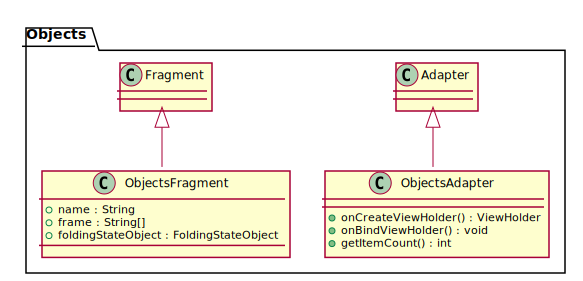
\includegraphics[width=0.70\linewidth]{../schemas/Conception_detaillee/classe_objects.pdf}
    \captionof{figure}{Diagramme du package Objects}
\end{minipage}

\subparagraph{Philosophie de conception \newline} 

\medspace

Le package Objects possède la classe ObjectAdapter du RecyclerView qui permet d'afficher la liste des objets. Elle permet de faire le lien entre les fragments et le RecyclerView. 
Chaque objet est matérialisé dans la liste des objets par une instance de la classe ObjectsFragment. 

\subparagraph{Description structurelle \newline}

\medspace

\textbf{Attributs :}

N.A.

\textbf{Services offerts :}

La classe ObjectAdapter contient les opérations suivantes : 

\begin{itemize}
    \item \textbf{onCreateViewHolder() : ViewHolder} --- Opération qui permet de créer un objet ViewHolder qui représente la vue d'un élément individuel dans le RecyclerView. 
    \item \textbf{onBindViewHolder() : void} --- Opération qui permet de lier les données d'un objet à la vue correspondante dans le RecyclerView. Elle est appelée lorsque le RecyclerView souhaite afficher ou mettre à jour les données d'un élément spécifique. 
    \item \textbf{getItemCount() : int} --- Opération qui permet de renvoyer le nombre total d'éléments dans la liste de données de l'adaptateur. Elle est utilisée par le RecyclerView pour déterminer combien d'éléments doivent être affichés.
\end{itemize}

\paragraph{La classe ObjectFragment}

\begin{minipage}
    {\linewidth}
    \centering
    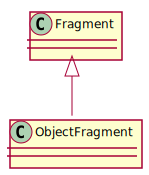
\includegraphics[width=0.40\linewidth]{../schemas/Conception_detaillee/classe_objectFragment.pdf}
    \captionof{figure}{Diagramme de classe de ObjectFragment}
\end{minipage}

\subparagraph{Philosophie de conception \newline} 

\medspace

La classe ObjectFragment est la classe associée à chaque fragment d'objet. Cette classe a pour rôle de créer un objet sur l'IHM et de lui associer ses trames.
Dans cette classe on détecte aussi si Utilisateur souhaite ajouter de nouvelles trames. 


\subparagraph{Description structurelle \newline}

\medspace

\textbf{Attributs :}

Les attribut associés à chaque objets sont : 
\begin{itemize}
    \item String name --- nom de l'objet
    \item String[] frame --- trames associées
    \item FoldingStateObject foldingStateObject --- état de l'objet (replié ou déplié)
\end{itemize}

\textbf{Services offerts :}

N.A.

\paragraph{L'énumération FoldingStateObject}

\begin{minipage}
    {\linewidth}
    \centering
    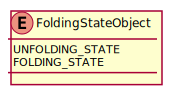
\includegraphics[width=0.40\linewidth]{../schemas/Conception_detaillee/classe_foldingStateObject.pdf}
    \captionof{figure}{Diagramme de l'énumération FoldingStateObject}
\end{minipage}

\subparagraph{Philosophie de conception \newline} 

\medspace

L'énumération FoldingStateObject permet de répertorier les deux états dans lesquels un objet peut être affiché. L'objet est visible sur l'écran, soit sous forme déplié (on peut observer les trames qu'il possède) soit sous forme replié (les potentielles trames qu'il possède ne sont pas visibles). Chaque objet visible sur l'écran possède cet attribut.

\subparagraph{Description structurelle \newline}

\medspace

\textbf{Attributs :}

N.A.

\textbf{Services offerts :}

\begin{itemize}
    \item \textbf{UNFOLDING\_STATE} --- Correspond à l'état déplié de l'objet (on observe les trames qu'il possède).
    \item \textbf{FOLDING\_STATE} --- Correspond à l'état replié de l'objet (les trames ne sont pas visibles).
\end{itemize}




